% filename: entropything.tex
\documentclass[tikz]{standalone}
\usepackage{tikz}

\begin{document}
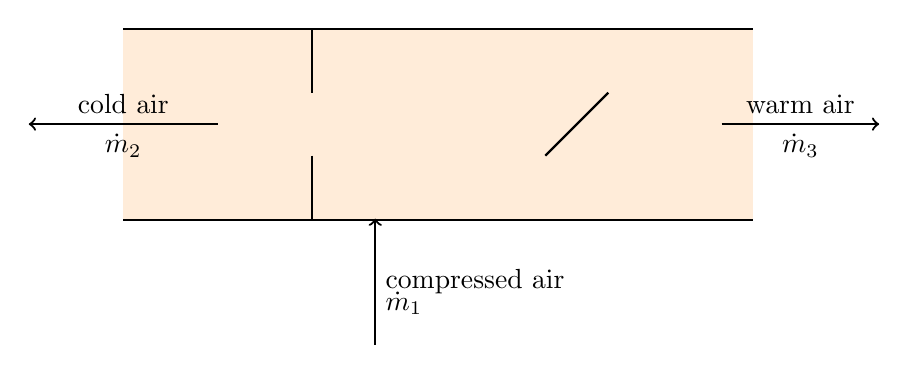
\begin{tikzpicture}[scale=0.8]
    \draw[thick, line width = 0.5mm] (2.5, 9.65) -- (12.5, 9.65);
    \draw[thick, line width = 0.5mm] (2.5, 6.65) -- (12.5, 6.65);
    \fill[orange!15!white] (2.5, 9.65) rectangle (12.5, 6.65);
    \draw[thick] (5.5, 9.65) -- (5.5, 8.65);
    \draw[thick] (5.5, 7.65) -- (5.5, 6.65);
    \draw[thick] (9.2, 7.65) -- (10.2, 8.65);
    \draw[thick, ->] (4.0, 8.15) -- (1.0, 8.15) node[midway, above]{cold air} node[midway, below]{$\dot{m}_2$};
    \draw[thick, ->] (12.0, 8.15) -- (14.5, 8.15)node[midway, above]{warm air} node[midway, below]{$\dot{m}_3$};;
    \draw[thick, ->] (6.5, 4.65) -- (6.5, 6.65)node[midway, right]{compressed air} node[midway, below right]{$\dot{m}_1$};;
\end{tikzpicture}
\end{document}